% This is a modified version of the tufte-latex book example in which the title page and the contents page resemble Tufte's VDQI book, using Kevin Godby's code from this thread at https://groups.google.com/forum/#!topic/tufte-latex/ujdzrktC1BQ.
%
%%%%%%%%%%%%%%%%%%%%%%%%%%%%%%%%%%%%%%%%%%%%%%%%%%%%%%%%%%%%%%%%%%%%%%
% How to use Overleaf: 
%
% You edit the source code here on the left, and the preview on the
% right shows you the result within a few seconds.
%
% Bookmark this page and share the URL with your co-authors. They can
% edit at the same time!
%
% You can upload figures, bibliographies, custom classes and
% styles using the files menu.
%
% If you're new to LaTeX, the wikibook is a great place to start:
% http://en.wikibooks.org/wiki/LaTeX
%
%%%%%%%%%%%%%%%%%%%%%%%%%%%%%%%%%%%%%%%%%%%%%%%%%%%%%%%%%%%%%%%%%%%%%%
%% Unfortunately for the contents to contain
%% the "Parts" lines successfully, hyperref
%% needs to be disabled.
\documentclass[nohyper, nobib]{tufte-book}
\usepackage{nameref}
% \hypersetup{colorlinks}% uncomment this line if you prefer colored hyperlinks (e.g., for onscreen viewing)

% \usepackage{hyphenat}
\usepackage{url}
\usepackage[backend=biber, natbib=true, style=numeric]{biblatex}
\usepackage{xargs}
\renewcommandx{\cite}[3][1={0pt},2={}]{\sidenote[][#1]{\fullcite[#2]{#3}}}
\usepackage{listings}

\definecolor{codegreen}{rgb}{0,0.6,0}
\definecolor{codegray}{rgb}{0.5,0.5,0.5}
\definecolor{almond}{rgb}{0.94, 0.87, 0.8}
\definecolor{antiquewhite}{rgb}{0.98, 0.92, 0.84}
\lstdefinestyle{mystyle}{ 
    commentstyle=\color{codegreen},
    keywordstyle=\color{magenta},
    backgroundcolor=\color{antiquewhite},
    basicstyle=\ttfamily\footnotesize,
    breakatwhitespace=false,         
    breaklines=true,                 
    captionpos=b,                    
    keepspaces=true,                 
    numbers=left,                    
    numbersep=5pt,                  
    showspaces=false,                
    showstringspaces=false,
}

\lstset{style=mystyle}
%%
% Book metadata
\title{Building Production Recommendation Systems in Python,\\ and JAX!}
% \date{The edition number}
\author{Bryan Bischof, Hector Yee}
\publisher{Publisher of This Book}

% Just some sample text
\usepackage{lipsum}

%%
% For nicely typeset tabular material
\usepackage{booktabs}

%%
% For graphics / images
\usepackage{graphicx}
\setkeys{Gin}{width=\linewidth,totalheight=\textheight,keepaspectratio}
\graphicspath{{graphics/}}

% The fancyvrb package lets us customize the formatting of verbatim
% environments.  We use a slightly smaller font.
\usepackage{fancyvrb}
\fvset{fontsize=\normalsize}

%%
% Prints argument within hanging parentheses (i.e., parentheses that take
% up no horizontal space).  Useful in tabular environments.
\newcommand{\hangp}[1]{\makebox[0pt][r]{(}#1\makebox[0pt][l]{)}}

%%
% Prints an asterisk that takes up no horizontal space.
% Useful in tabular environments.
\newcommand{\hangstar}{\makebox[0pt][l]{*}}

%%
% Prints a trailing space in a smart way.
\usepackage{xspace}

%%
% Some shortcuts for Tufte's book titles.  The lowercase commands will
% produce the initials of the book title in italics.  The all-caps commands
% will print out the full title of the book in italics.
\newcommand{\vdqi}{\textit{VDQI}\xspace}
\newcommand{\ei}{\textit{EI}\xspace}
\newcommand{\ve}{\textit{VE}\xspace}
\newcommand{\be}{\textit{BE}\xspace}
\newcommand{\VDQI}{\textit{The Visual Display of Quantitative Information}\xspace}
\newcommand{\EI}{\textit{Envisioning Information}\xspace}
\newcommand{\VE}{\textit{Visual Explanations}\xspace}
\newcommand{\BE}{\textit{Beautiful Evidence}\xspace}

\newcommand{\TL}{Tufte-\LaTeX\xspace}

% Prints the month name (e.g., January) and the year (e.g., 2008)
\newcommand{\monthyear}{%
  \ifcase\month\or January\or February\or March\or April\or May\or June\or
  July\or August\or September\or October\or November\or
  December\fi\space\number\year
}


% Prints an epigraph and speaker in sans serif, all-caps type.
\newcommand{\openepigraph}[2]{%
  %\sffamily\fontsize{14}{16}\selectfont
  \begin{fullwidth}
  \sffamily\large
  \begin{doublespace}
  \noindent\allcaps{#1}\\% epigraph
  \noindent\allcaps{#2}% author
  \end{doublespace}
  \end{fullwidth}
}

% Inserts a blank page
\newcommand{\blankpage}{\newpage\hbox{}\thispagestyle{empty}\newpage}

\usepackage{units}

% Typesets the font size, leading, and measure in the form of 10/12x26 pc.
\newcommand{\measure}[3]{#1/#2$\times$\unit[#3]{pc}}

% Macros for typesetting the documentation
\newcommand{\hlred}[1]{\textcolor{Maroon}{#1}}% prints in red
\newcommand{\hangleft}[1]{\makebox[0pt][r]{#1}}
\newcommand{\hairsp}{\hspace{1pt}}% hair space
\newcommand{\hquad}{\hskip0.5em\relax}% half quad space
\newcommand{\TODO}{\textcolor{red}{\bf TODO!}\xspace}
\newcommand{\ie}{\textit{i.\hairsp{}e.}\xspace}
\newcommand{\eg}{\textit{e.\hairsp{}g.}\xspace}
\newcommand{\na}{\quad--}% used in tables for N/A cells
\providecommand{\XeLaTeX}{X\lower.5ex\hbox{\kern-0.15em\reflectbox{E}}\kern-0.1em\LaTeX}
\newcommand{\tXeLaTeX}{\XeLaTeX\index{XeLaTeX@\protect\XeLaTeX}}
% \index{\texttt{\textbackslash xyz}@\hangleft{\texttt{\textbackslash}}\texttt{xyz}}
\newcommand{\tuftebs}{\symbol{'134}}% a backslash in tt type in OT1/T1
\newcommand{\doccmdnoindex}[2][]{\texttt{\tuftebs#2}}% command name -- adds backslash automatically (and doesn't add cmd to the index)
\newcommand{\doccmddef}[2][]{%
  \hlred{\texttt{\tuftebs#2}}\label{cmd:#2}%
  \ifthenelse{\isempty{#1}}%
    {% add the command to the index
      \index{#2 command@\protect\hangleft{\texttt{\tuftebs}}\texttt{#2}}% command name
    }%
    {% add the command and package to the index
      \index{#2 command@\protect\hangleft{\texttt{\tuftebs}}\texttt{#2} (\texttt{#1} package)}% command name
      \index{#1 package@\texttt{#1} package}\index{packages!#1@\texttt{#1}}% package name
    }%
}% command name -- adds backslash automatically
\newcommand{\doccmd}[2][]{%
  \texttt{\tuftebs#2}%
  \ifthenelse{\isempty{#1}}%
    {% add the command to the index
      \index{#2 command@\protect\hangleft{\texttt{\tuftebs}}\texttt{#2}}% command name
    }%
    {% add the command and package to the index
      \index{#2 command@\protect\hangleft{\texttt{\tuftebs}}\texttt{#2} (\texttt{#1} package)}% command name
      \index{#1 package@\texttt{#1} package}\index{packages!#1@\texttt{#1}}% package name
    }%
}% command name -- adds backslash automatically
\newcommand{\docopt}[1]{\ensuremath{\langle}\textrm{\textit{#1}}\ensuremath{\rangle}}% optional command argument
\newcommand{\docarg}[1]{\textrm{\textit{#1}}}% (required) command argument
\newenvironment{docspec}{\begin{quotation}\ttfamily\parskip0pt\parindent0pt\ignorespaces}{\end{quotation}}% command specification environment
\newcommand{\docenv}[1]{\texttt{#1}\index{#1 environment@\texttt{#1} environment}\index{environments!#1@\texttt{#1}}}% environment name
\newcommand{\docenvdef}[1]{\hlred{\texttt{#1}}\label{env:#1}\index{#1 environment@\texttt{#1} environment}\index{environments!#1@\texttt{#1}}}% environment name
\newcommand{\docpkg}[1]{\texttt{#1}\index{#1 package@\texttt{#1} package}\index{packages!#1@\texttt{#1}}}% package name
\newcommand{\doccls}[1]{\texttt{#1}}% document class name
\newcommand{\docclsopt}[1]{\texttt{#1}\index{#1 class option@\texttt{#1} class option}\index{class options!#1@\texttt{#1}}}% document class option name
\newcommand{\docclsoptdef}[1]{\hlred{\texttt{#1}}\label{clsopt:#1}\index{#1 class option@\texttt{#1} class option}\index{class options!#1@\texttt{#1}}}% document class option name defined
\newcommand{\docmsg}[2]{\bigskip\begin{fullwidth}\noindent\ttfamily#1\end{fullwidth}\medskip\par\noindent#2}
\newcommand{\docfilehook}[2]{\texttt{#1}\index{file hooks!#2}\index{#1@\texttt{#1}}}
\newcommand{\doccounter}[1]{\texttt{#1}\index{#1 counter@\texttt{#1} counter}}

% Generates the index
\usepackage{makeidx}
\makeindex

%%%% Kevin Godny's code for title page and contents from https://groups.google.com/forum/#!topic/tufte-latex/ujdzrktC1BQ
\makeatletter
\renewcommand{\maketitlepage}{%
\begingroup%
\setlength{\parindent}{0pt}

{\fontsize{24}{24}\selectfont\textit{\@author}\par}

\vspace{1.75in}{\fontsize{36}{54}\selectfont\@title\par}

\vspace{0.5in}{\fontsize{14}{14}\selectfont\textsf{\smallcaps{\@date}}\par}

\vfill{\fontsize{14}{14}\selectfont\textit{\@publisher}\par}

\thispagestyle{empty}
\endgroup
}
\makeatother

\titlecontents{part}%
    [0pt]% distance from left margin
    {\addvspace{0.25\baselineskip}}% above (global formatting of entry)
    {\allcaps{Part~\thecontentslabel}\allcaps}% before w/ label (label = ``Part I'')
    {\allcaps{Part~\thecontentslabel}\allcaps}% before w/o label
    {}% filler and page (leaders and page num)
    [\vspace*{0.5\baselineskip}]% after

\titlecontents{chapter}%
    [4em]% distance from left margin
    {}% above (global formatting of entry)
    {\contentslabel{2em}\textit}% before w/ label (label = ``Chapter 1'')
    {\hspace{0em}\textit}% before w/o label
    {\qquad\thecontentspage}% filler and page (leaders and page num)
    [\vspace*{0.5\baselineskip}]% after
    
%%%% End additional code by Kevin Godby

\begin{document}

% Front matter
\frontmatter

% r.3 full title page
\maketitle

% v.4 copyright page
\newpage
\begin{fullwidth}
~\vfill
\thispagestyle{empty}
\setlength{\parindent}{0pt}
\setlength{\parskip}{\baselineskip}
Copyright \copyright\ \the\year\ \thanklessauthor

\par\smallcaps{Published by \thanklesspublisher}

\par\smallcaps{tufte-latex.googlecode.com}

\par Licensed under the Apache License, Version 2.0 (the ``License''); you may not
use this file except in compliance with the License. You may obtain a copy
of the License at \url{http://www.apache.org/licenses/LICENSE-2.0}. Unless
required by applicable law or agreed to in writing, software distributed
under the License is distributed on an \smallcaps{``AS IS'' BASIS, WITHOUT
WARRANTIES OR CONDITIONS OF ANY KIND}, either express or implied. See the
License for the specific language governing permissions and limitations
under the License.\index{license}

\par\textit{First printing, \monthyear}
\end{fullwidth}

% r.5 contents
\tableofcontents

% \listoffigures

% \listoftables


\chapter*{Preface}

How did you come to find this book? Did you see an ad for it on some website? Maybe a friend or instructor suggested it; or perhaps you saw a tweet referencing it. Could it be that you found it sitting on a shelf in a bookstore; a bookstore that your trusty maps app led you to. In any case, you’ve almost certainly come to this book via a recommendation system.

Implementing and designing systems to provide suggestions to users is among the most popular and most essential first applications of Machine Learning to any business. Whether you wish to help your users find the best clothing to their tastes, the most appealing items to buy from your online store, the videos to enrich and entertain them, maximally engaging content from their networks, or the news they need to know on that day, recommendation systems(often abbreviated RecSys) provide the way.

Modern recommendation system designs are as diverse as the fields in which they serve. Methods for recommending can come from traditional statistical learning algorithms, linear algebraic inspirations, geometric considerations, and, of course, gradient based methods. While the algorithmic methods are diverse, so too are the statistical and evaluation considerations for recommending: personalized ranking, search recommendations, sequence modeling, and the scoring for all of the above are now need-to-know for the working ML Engineer in the space of recommendation systems.

As a practitioner, you’ll need to understand:
\begin{itemize}
    \item What are the essential data to get started building a RecSys
    \item How to take your data and business problem, and frame it as a RecSys problem
    \item What are the appropriate models for your RecSys problem and how should you evaluate them
    \item How to implement, train, test, and deploy the aforementioned model
    \item What metrics you should be tracking to ensure your system is working as planned
    \item How to incrementally improve your system as you learn more about your users, products, and business case
\end{itemize}

This book seeks to illustrate the core concepts and examples necessary to do the above–whatever the industry or scale. In this book we guide the reader through the math, ideas, and implementation details of your first or fiftieth recommendation system. We illustrate how to build these systems with Python and JAX.

% r.9 introduction
\cleardoublepage

%%
% Start the main matter (normal chapters)
\mainmatter

\part{The Warmup}

\chapter{Definition and Introduction}
\label{ch:introduction}

\section{What on earth are we doing here?}

Ubiquity of any technology often prompts questions of how the technology works, why it has become so common, and if one can get in on the action. For recommendation systems, the how is quite complicated. 

Most machine learning practitioners are aware of recommendation systems, many can tell you one or two of the simplest modeling approaches, and some can speak intelligently about the relevant data structures and model architectures; however, RecSys*(what practitioners call the field, and sometimes the systems themselves)* frequently falls outside the core curriculum of Data Science and Machine Learning. Many a senior Data Scientist with years of experience in the industry knows little about actually building a recommendation system, and may feel intimidated when they came up. Despite drawing on similar foundations and skills as other Machine Learning problems, RecSys has a vibrant and fast moving community that can make it easy to relegate building recommendation systems to *other* Data Scientists.

The reason this book exists, is to break through that disinclination. Understanding recommendation systems at a practical level is not only useful for business cases where content needs to be served to users, but the underlying ideas of RecSys often bridge gaps between an incredibly diverse set of other types of Machine Learning. Even more excitingly, no matter what aspects of mathematics one finds themselves interested in, sooner or later, there appears a link or application in RecSys! Finally, if connections to other fields, applications of nearly all of mathematics, or the obvious business utility *aren't* enough to get you interested in RecSys, the stunning cutting edge technology might. RecSys is at and beyond the forefront of Machine Learning at all times–one benefit of having very obvious revenue impact is that companies and practitioners need to always be pushing the boundaries of what is possible, and how they go about it. The most advanced Deep Learning architectures and best code infrastructures are brought to bear on this field. Hardly a surprise when you consider that at the heart of 4 of the 5 letters in FAANG, lies one or many recommendation systems.

We will formulate a number a variants of the core problem of recommendation systems, but at it's core the motivating problem framing is:


Given a collection of things that may be recommended, choose an ordered few for the current context and user that best match according to some objective.


\section{What are the key components of a RecSys?}

As we increase complexity and sophistication, let's keep in mind what the components of our system are. We will use what are called *string diagrams* to keep track of the different components, but in the literature a variety of presentations of these diagrams appear.

\begin{enumerate}
    \item Collector
    \item Ranker
    \item Server
\end{enumerate}


\subsection{Collector}

The collector's role is to know what is in the collection of things that may be recommended, and the necessary features or attributes of those things.

\subsection{Ranker}

The ranker's role is to take the collection provided by the collector, and order some or all of them, according to a model for the context and user.

\subsection{Server}

The server's role is to take the ordered subset provided by the ranker, ensure that the necessary data schema is satisfied–including essential business logic–and return the requested number of recommendations. 

\begin{quote}
    Take, for example, a hospitality scenario with a waiter. When you sit down at your table, you look at the menu unsure of what you should order. You ask to the wait staff, "what do you think I should order for dessert?"
    
    The waiter checks their notes and says "we're out of the key lime pie, but people really like our banana creme pie. If you like pomegranate, we make pom ice-cream from scratch; and it's hard to go wrong with the donut a la mode–it's our most popular dessert."
\end{quote} 


In this short exchange, the waiter first serves as a collector; they identify the desserts on the menu, accommodate current inventory conditions by checking their notes, and finally prepare themselves to talk about the characteristics of the desserts.

Next, the serve as a ranker; they mention items both high scoring in popularity (banana creme pie and donut a la mode), and a contextually high match item based on the patron's features (if they like pomegranate).

Finally, they serve the recommendations verbally, including both explanatory features of their algorithm and multiple choices. 

While this seems a bit cartoonish, remember to ground later discussions of recommender systems in real world applications. One of the advantages of working in recommendation systems is that inspiration is always near by.

\section{What is the simplest possible recommender?}

\subsection{The trivial recommender}

The absolute simplest recommender is not very interesting, but may still be demonstrated in the above framework. It's called \emph{the trivial recommender (TR)} because it contains virtually no logic:

\begin{lstlisting}[language=Python]
def get_trivial_recs() -> Optional[List[str]]:
    if get_availability(ITEM_ID):
        return [ITEM_ID]
    return None
\end{lstlisting}


Notice that this recommender may either return a specific \lstinline{ITEM_ID} or \lstinline{None}. Also observe that this recommender takes no arguments, and \lstinline{ITEM_ID} is referencing a variable out-of-scope. Software principles ignored, let's think about the three components:
\begin{itemize}
    \item Collector: The TR collects by checking the availability of \lstinline{ITEM_ID}. One could argue that having access to \lstinline{ITEM_ID} is also part of the collector's responsibility. Conditional upon the availability, the collection of recommendable things is either \lstinline{[ITEM_ID]} or \lstinline{None} (recall that \lstinline{None} is a collection in the set-theoretic sense).
    \item Ranker: The TR ranks with a no-op; i.e. the ranking of 1 or 0 objects in a collection is the identity function on that collection, so we merely do nothing and move onto the next step.
    \item Server: The TR serves recommendations by its return statements. The only schema that's been specified above, is that the return type is \lstinline{Optional[List[str]]}. 

\end{itemize}

We certainly would not expect the above recommender to be interesting or useful, but it provides a skeleton which we will add to as we develop further.

\subsection{Most-popular-item recommender}

The \emph{most-popular-item recommender (MPIR)} is the simplest recommender that contains much or any utility. It works, just as it says: it returns the most popular items.

\begin{lstlisting}[language=Python]
def get_item_popularities() -> Optional[Dict[str, int]]:
    ...
        # Dict of pairs: (item-identifier, count item chosen)
        return item_choice_counts 
    return None

def get_most_popular_recs(max_num_recs: int) -> Optional[List[str]]:
    items_popularity_dict = get_item_popularities() # type: Optional[Dict[str, int]]
    if items_popularity_dict:
        sorted_items = sorted(
            items_popularity_dict.items(), 
            key=lambda item: item[1]),
            reverse=True,
        )
        return [i[0] for i in sorted_items][:max_num_recs]
    return None
\end{lstlisting}


Here we assume that \lstinline{get_item_popularities} has knowledge of all available items and how many times they've been chosen.

As is probably obvious; this recommender attempts to return the `k` most popular items which are available. While simple, this is a very useful recommender that serves as a great place to start when building a recommendation system. Additionally, we will see this example return over and over, because other recommenders use this core and simply improve the internal components.

\subsection{Collector}

The MPIR first makes a call to \lstinline{get_item_popularities} which, via database or memory access, knows which items are available, and how many time they've been selected. For convenience, we assume that they're returned as a dictionary with keys the item-identifier string, and values the number of times that item has been chosen. We implicitly assume here that items not appearing in this list are not available.

\subsection{Ranker}

Here we see our first simple ranker: ranking by sorting on values. Because the collector has organized our data such that the values of the dictionary are the counts, we use the python built-in sorting function `sorted`. Note that we use the `key` to indicate that we wish to sort by the second element of the tuples–in this case equivalent to sorting by values–and we send the reverse flag to make our sort descending.

\subsection{Server}

Finally, we need to satisfy our API schema, which is again provided via the return type hint: \lstinline{Optional[List[str]]}. This wants the return type to be the nullable list of item-identifier strings that we're recommending, so we use a list comprehension to grab the first element of the tuples. But wait! Our function has this \lstinline{max_num_recs} field–what might that be doing there? Of course, this is suggesting that our API schema is looking for no greater than \lstinline{max_num_recs} in the response. We handle this via the slice operator, but take note that our return is between 0 and \lstinline{max_num_recs} results.

---

While we've not done much math yet, we have gotten to the point where we may begin providing recommendations and implementing deeper logic into these components. We'll start doing things that look like machine learning soon enough.




\chapter{User/Item ratings and framing the problem}
\label{ch:user-item}

\section{The user-item matrix}

It's extremely common to hear those who work on Recommendation Systems, talk about matrices, and in particular the user-item matrix. While linear algebra is deep, both mathematically and as it applies to RecSys, we actually will begin with very simplistic relationships. 

Before we get to the matrix forms, let's write down some binary relationships between a set of users and a set of items. For the sake of this example, think of a group of 5 friends (mysteriously named 'A', 'B', 'C', 'D', 'E') and a blind cheese tasting where they're trying out four different cheeses, 'W', 'X', 'Y', 'Z', . The friends are asked to rate the cheeses, 1-5:
\begin{itemize}
    \item \colorbox{almond}{\parbox{\textwidth-10pt}{
 A starts,  "Ok, I really enjoy W, give that a 5, X \& Y are yummy too, 4, and Z is awful, 1."
}}
    \item \colorbox{almond}{\parbox{\textwidth-10pt}{
 B replies, "what?! Z is my favorite! 4.5! X \& Y are fine, 3, and W is just ok, 2."
}}
    \item \colorbox{almond}{\parbox{\textwidth-10pt}{
 B replies, "what?! Z is my favorite! 4.5! X \& Y are fine, 3, and W is just ok, 2."
}}
    \item \colorbox{almond}{\parbox{\textwidth-10pt}{
 D gives 4,4,5, but we run out of Z before D can try it. 
}}
    \item \colorbox{almond}{\parbox{\textwidth-10pt}{
 E starts to feel not well, and only tries "W" giving it a 3.
}}
\end{itemize}

The first thing you may notice is that this is a bit annoying to read and parse out. Almost immediately you may want to write this in a more compact and convenient form. Like a collection of lists:

\begin{center}
\begin{math}
\begin{array}{cc}
    A:[5,4,4,1] \\
    B:[2,3,3,4.5] \\
    C:[3,2,3,4] \\
    D:[4,4,5,-] \\
    E:[3,-,-,-] \\
\end{array}
\end{math}
\end{center}
This is relatively ok, but you might want to more clearly indicate the positional meaning in each list:

\begin{lstlisting}[language=Python]
_ = np.nan
scores = np.array([[5,4,4,1],
    [2,3,3,4.5],
    [3,2,3,4],
    [4,4,5,_],
    [3,_,_,_]])
sns.heatmap(
    scores, 
    annot=True, 
    fmt=".1f", 
    xticklabels=['W','X','Y','Z',], 
    yticklabels=['A','B','C','D','E',]
)
\end{lstlisting}

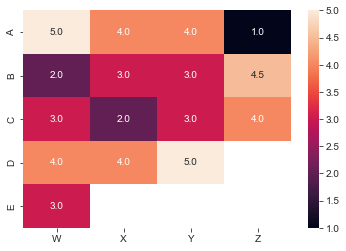
\includegraphics[width=\textwidth-20pt]{book-text/ratings_heatmap.png}

A few natural questions emerge:

\begin{enumerate}
\item What's the most popular cheese? From the observations so far, it's looking like Y is potentially the favorite, but E didn't try Y. 
\item Would D like cheese Z? It seems to be a contentious cheese.
\item If we were asked to buy two cheeses only, which should we buy to satisfy everyone the most?
\end{enumerate}

... and so on. This is cartoonish, and small, but I think the point is clear that this matrix representation above is at least convenient for capturing these ratings.

What may not come obviously is that beyond the convenience of this data visualization, is the mathematical utility of this representation. Question 2 above posits a question that is inherent in the RecSys problem space: "predict how much a user will like an item they've not seen". This question also may be recognizable as a problem from a linear algebra class: "how can we fill in unknown elements of a matrix from the ones we know". This is what is called \emph{matrix completion.}

Before we dive into the linear algebra, let's consider the purely data science perspective called collaborative filtering ([Goldeberg et al, '92](\url{https://d2l.ai/chapter_references/zreferences.html#goldberg-nichols-oki-ea-1992})). The underlying idea is that those with similar taste, help others to know what they like without them having to try it themselves. The collaboration aspect was originally intended to mean among similar-taste users, and the filtering aspect was originally intended to mean filtering out things people wont like.

\section{User-user vs item-item CF}

There are two ways to think of this collaborative filtering strategy:
\begin{itemize}
    \item Two users with similar taste, will continue to have similar taste
    \item Two items with similar user fans, will continue to be popular with other similar users
\end{itemize}

It may sound like these are identical, but perhaps surprisingly, they appear differently in the mathematical interpretations. At a high level, the difference is deciding which kind of similarity do you wish your recommender to make priority of–user similarity or item similarity.

If you prioritize user similarity, then to provide a recommendation for a user $A$, you find a similar user $B$, and then choose a recommendation from $B$'s list of liked content that $A$ hasn't seen  for $A$. 

If you prioritize item similarity, then to provide a recommendation for a user $A$, you find an item that $A$ liked $X$, then you find an item similar to $X$ that $A$ hasn't seen, $Y$, and recommend it for $A$.

Later we will dive deeper into similarity, but let's quickly link these ideas to our brief discussion above. Similar users are rows of the user-item matrix which are similar as vectors; similar items are columns of the user-item matrix which are similar as vectors.


\vspace{10pt}
\colorbox{almond}{\parbox{\textwidth}{
 \emph{Vector similarity} will be more precisely define later, for now, consider similarity to be computed by normalizing the vectors, and then taking their cosine similarity.
}}
\vspace{10pt}


\subsection{The Netflix challenge}

In 2006, an online competition was kicked off on the website \url{www.thenetflixprize.com}. This competition, was to see if teams could improve on the performance of the Netflix team's collaborative filtering algorithms on an open sourced dataset from the company. While this is more common today via websites like Kaggle or via conference competitions, it was very exciting for those interested in RecSys.

The competition consisted of several intermediate rounds of what were called Progress Prize, and the final Netflix Prize was awarded in 2009. The data provided was a collection of 2,817,131 triples consisting of \lstinline{(user, movie, date_rated)}. And half of these additionally include the rating itself. Notice that like our above example, the user-item information is nearly enough to specify the problem. In this particular dataset, the date was provided. Later on, we will dig into how time might be a factor, and in particular, sequential recommendation systems. 

The stakes were quite high in this competition, requirements for beating the internal performance were a 10\% increase in RMSE (we will discuss this loss function later), but the spoils added up to over \$1.1M. The final winners were BellKor's Pragmatic Chaos(who incidentally one the two previous Progress prizes) with a test RMSE of $0.8567$. In the end, only a $20$-min earlier submission kept BellKor ahead of the competitors The Ensemble. 

c.f. 
\begin{itemize}
\item \url{https://www.researchgate.net/publication/223460749_The_BigChaos_Solution_to_the_Netflix_Grand_Prize}

\item \url{https://www2.seas.gwu.edu/~simhaweb/champalg/cf/papers/ProgressPrize2008_BigChaos.pdf}
\end{itemize}
There are a number of important lessons to be learned from this game, but for the sake of brevity:

\begin{itemize}
\item the user-item matrix is at the heart of collaborative filtering and more generally specifying RecSys problems
\item parameter tuning provided a huge improvement in several algorithms
\item several model innovations came from thinking very hard about the business use-case and human behavior
\item linear algebraic approaches served not only as the first reasonably performant solutions, but building on top of them led to the ultimately winning approach
\item eking out the performance that Netflix originally demanded to win the competition too so long, that business circumstances changed, and the [solution was no longer useful]\url{https://thenextweb.com/news/remember-netflixs-1m-algorithm-contest-well-heres-why-it-didnt-use-the-winning-entry}.
\end{itemize}

That last one might be the \lstinline{most} important thing a machine learning developer needs to learn about recommendations systems: build a working usable model quickly and iterate while the business still cares.


\section{Soft ratings}

In our example above, each cheese received either a numerical rating, or was not tried by a guest. These are what are called **hard ratings**–regardless if the cheese is a brie or a chevre; they are explicit, and their absence indicates a lack of interaction between the user and item. In some contexts, we wish to accommodate circumstances wherein a user does interact with an item, and yet no rating is provided.

A common example is a movies app; a user may have watched a movie with the app, but not provided a star rating. This indicates that the item–in this case a movie–has been observed, but we don't have the rating for our algorithms to learn from. However, we can still make use of this implicit data:

\begin{itemize}
\item we can exclude this item from future recommendations
\item we could separately use this data as a separate term in our learner
\item we could assign a default rating value to indicate "interesting enough to watch, not significant enough to rate"
\end{itemize}

It turns out that implicit ratings are very important for training effective recommendation systems, not only because it's common that users don't give hard ratings, but because they provide a different level of signal. Later, when we wish to train multi-level models to predict both click-likelihood and buy-likelihood, these two levels will prove extremely important.

\section{Data collection and user-tracking}

We established above that we learn both from explicit ratings and implicit ratings, so how and where do we get this data? To dive into this, we'll need to start worrying about application code. In many businesses, the data scientists and ML engineers are separate from the engineers, but for recommendation systems, there's a strong need for alignment between the two functions.

\subsection{What to track}

The simplest and most obvious data collection is user-ratings. If users are given the option to provide ratings or even thumbs-up and thumbs-down, that component will need to be built and that data will be stored. These ratings must be stored not only for the opportunity to build recommendations, it's also a bad user experience to rate something and then shortly thereafter the rating doesn't appear if you revisit the page.

Similarly, it's useful to understand a few other key interactions that we will see can improve and expand your RecSys: \lstinline{page loads}, \lstinline{page views}, \lstinline{clicks}, and \lstinline{add-to-bag}.

For these data, let's use a slightly more complicated example, an e-commerce website. Let's take for this example www.bookshop.org. There are many different applications of RecSys on this one page, almost all of which we will return to in time, but for now let's focus on some interactions.

\vspace{10pt}
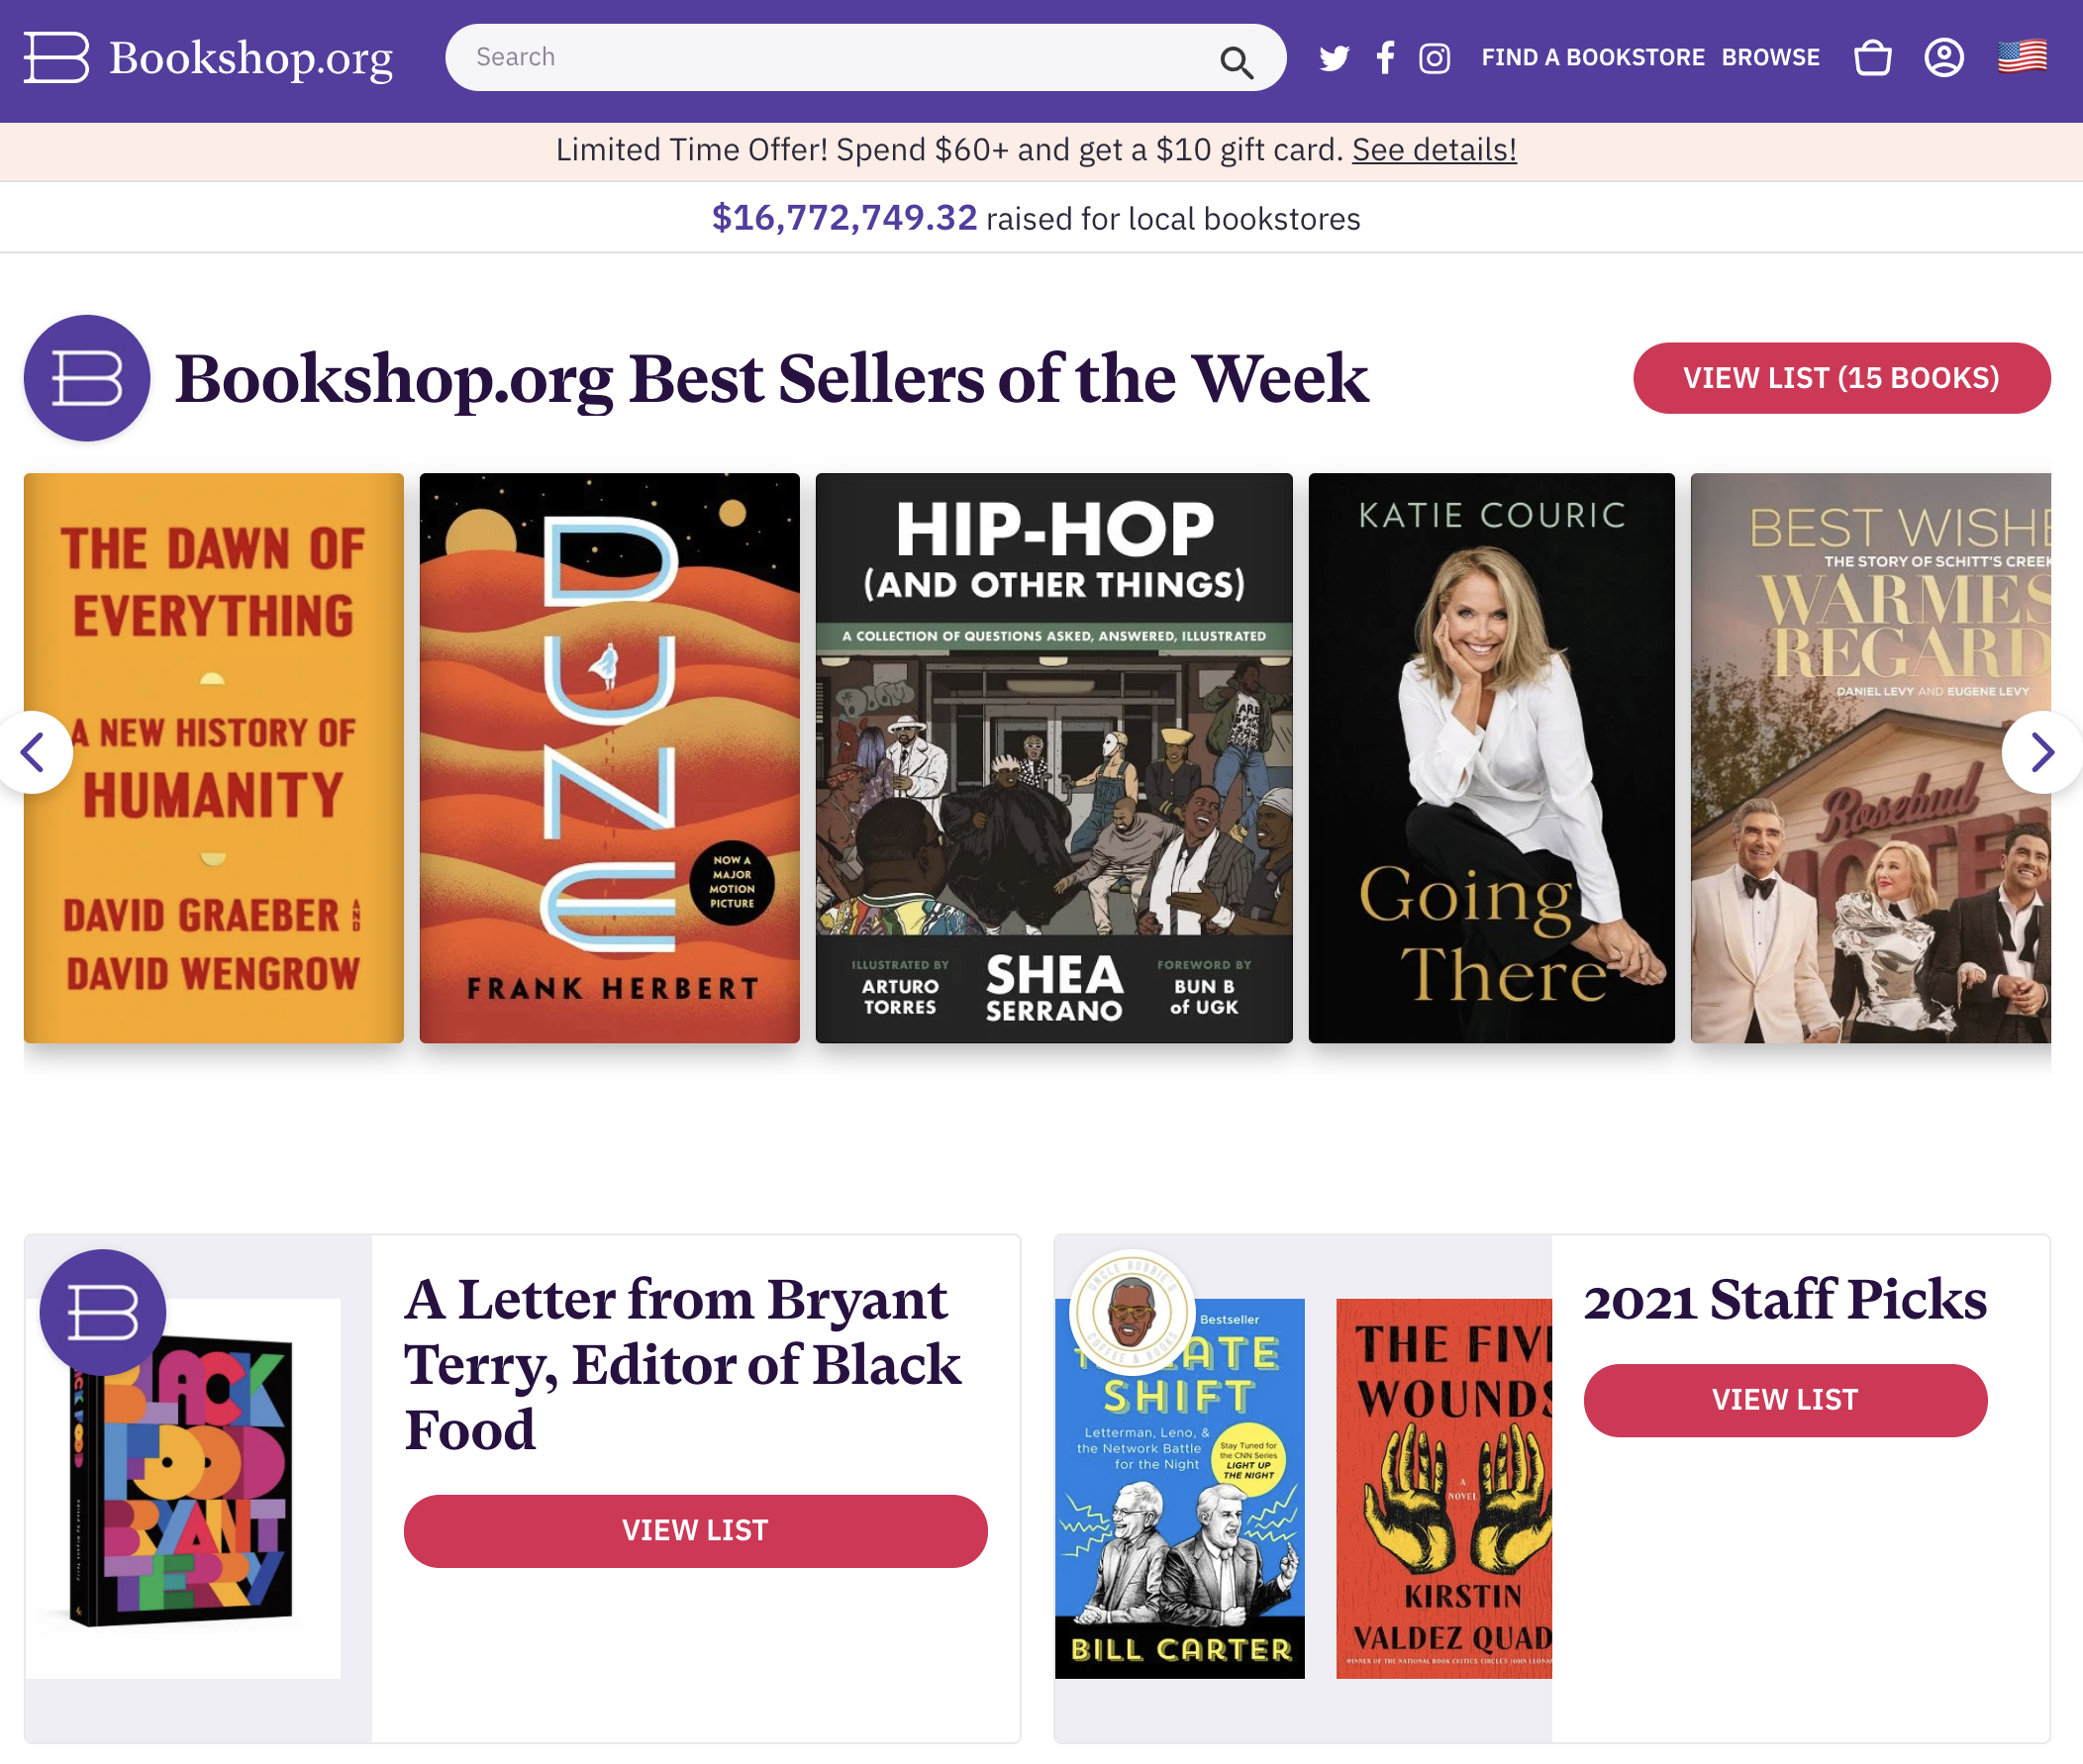
\includegraphics[width=\textwidth-10pt]{book-text/bookshop-landingpage.png}

\paragraph{Page Loads}

When you first load up Bookshop, it starts with items on the page. In the above screenshot, the \emph{Best Sellers of the Week} are all clickable images to those book listings. Despite the user having no choice in this initial page, it's actually quite important to log what is contained in this initial page load. 

These options provide the population of books that the user has seen. If a user has seen an option, then they have the opportunity to click on it, which will ultimately be an important implicit signal. 


\vspace{10pt}
\colorbox{almond}{\parbox{\textwidth}{ This notion is deeply tied to **propensity score matching;** in mathematics, propensity scores are the probability that an observational unit will be assigned to the treatment vs. the control.
}}
\vspace{10pt}

Compare this to the simple 50-50 A/B test: every unit has a 50\% chance of being exposed to your treatment. In a feature-stratified A/B test, you purposely change the probability of exposure dependent on some feature or collection of features (often called covariates in this context). Those probability of exposures are the propensity scores. 

So why bring up A/B testing here? Later, we'll be interested in mining our soft ratings for signal on user preference, but we must consider the possibility that the lack of a soft rating, is not an implicit bad rating. Thinking back to the cheeses: taster D never had a chance to rate Z, so there's no reason to think D has a preference or aversion in Z. This is because D was not **exposed to Z.** Now thinking back to Bookshop: the page above does not show The Hitchhiker's Guide to the Galaxy, so I have no way to click on it, and thus implicitly communicate that I'm interested in that book. I could use the search, but that's a different kind of signal(which we'll talk about later and, in fact, is a much stronger signal).

When understanding implicit ratings like "did the user look at something" we need to properly account for the entire population of things they were exposed to, and use the inverse of that population size to weight the importance of clicking. For this reason, understanding *all* page loads is important.

\paragraph{Page views and hover}

Websites have gotten much more complicated, and now there are a variety of interactions one must contend with. Look what happens if I click the right arrow in the \emph{Best Sellers of the Week} carousel and then move my mouse over the \emph{Cooking at Home} option:


\vspace{10pt}
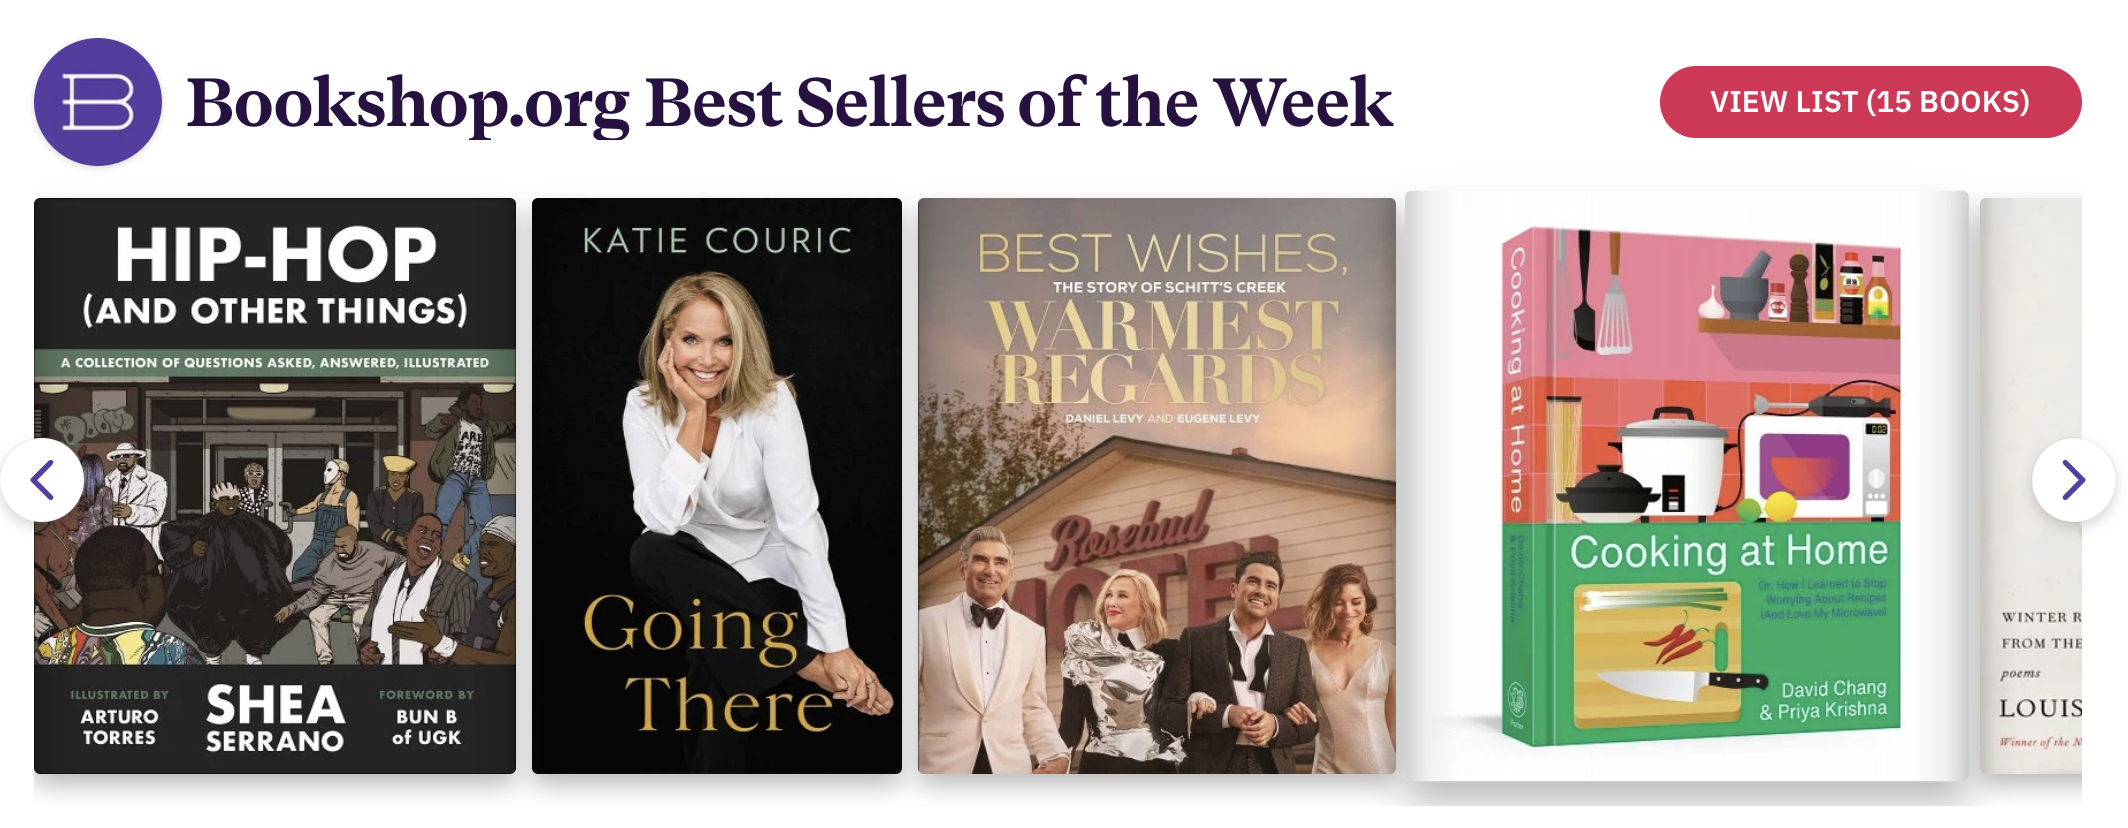
\includegraphics[width=\textwidth-10pt]{book-text/bookshop-top-sellers.png}

I've unveiled a new option, and mousing over it, made it larger and have a visual effect. These are ways to communicate to the user more information, and remind the user that these are clickable. To the recommender, these can be used as more implicit feedback.

First, the user clicked the carousel scroll–so some of what they saw in the carousel was interesting enough to dig further. Second, they moused over *Cooking at Home* they might click, or they might just want to see if there's additional information when hovering. Many websites use a hover interaction to provide a pop-up detail. While bookshop doesn't implement something like this; internet users have been trained to expect this behavior by all the websites that do, and so the signal is still meaningful. Third, they've now uncovered a new potential item in their carousel scroll–something we should add to our page loads, but really should come with a higher rating because it required interaction to uncover. 

All this and more can be encoded into the website's logging, rich and verbose logging is one of the most important thing to improve a recommendation system, and it's almost always better to have more than you need rather than the opposite.

\paragraph{Clicks}

If you thought hovering meant interest, wait until you hear about clicking! Not in all cases, but in the large majority, clicking is a very strong indicator of product interest. For e-commerce, clicking often is computed as part of the recommendation team's core KPIs (key performance indicators). 

This is for two reasons:

\begin{itemize}
\item clicking is almost always required to purchase; so it's an upstream filter for all business transactions
\item clicking requires explicit user action; so it's a good measure of intent
\end{itemize}

There will always be noise of course, but clicks are the go-to indicator of what a client is interested in. Many production recommendation systems are trained on click data–not ratings data–because of the much higher data volume and because of strong correlation between click behavior and purchase behavior. 


\vspace{10pt}
\colorbox{almond}{\parbox{\textwidth}{ Sometimes in Recommendation Systems you hear people talk about 'click-stream' data. It is an important view into clicks data, that also considers the order of a users click in a single 'session'. Modern recommendation systems put a lot of effort into utilizing the order of items a user clicks on, calling this sequential recommendations, and have show dramatic improvements via this additional dimension. We will discuss sequence-based recs later in the book.
}}
\vspace{10pt}

\paragraph{Add to bag}

We've finally arrived, the user has added some item to their bag or cart or queue. This is an extremely strong indicator of interest, and is often very strongly correlated with purchasing. There are even reasons to argue that add-to-bag is a better signal than purchase/order/watch. Add-to-bag is essentially the end of the line for soft ratings, and usually beyond this you'd want to start collecting ratings and reviews.


\paragraph{Collection and instrumentation}

Web applications very frequently instrument all of the above via 'events'. If you don't yet know what events are, maybe ask a buddy in your engineering org–but we'll give you the skinny. Like logging, events are specially formatted message that the application sends out when a certain block of code is executed. Like in the example of a click, the application needs to make a call to get the next content to show the user. It's common to also "fire an event" at this moment indicating information about the user, what they clicked on, the session id for later reference, the time, and various other useful things. This event can be handled downstream in any number of ways, but there's a increasingly possible pattern of it's path bifurcating to:

\begin{itemize}
\item a log database, like a mysql application database tied to the service
\item an event stream for real-time handling
\end{itemize}

The latter is actually what's interesting to us here. Event streams are often connected up to listeners via technologies like Kafka. This kind of infrastructure can get complicated fast (consult your local data engineer or devOps person), but a simple model for what happens is that all of a particular kind of log are sent to a bunch of different destinations that you think can make use of these events.

In the recommender case, an event stream can be connected up to some transformations to process the data for downstream learning tasks. This will be enormously useful if you want to build a recommendation system that uses those logs. Other important uses are real-time metrics tracking for what's going on at any given time on the website.

\subsection{Aside: Funnels}

We've just worked through our first example of a funnel, and no good Data Scientist can avoid thinking about funnels at some point. Like them or hate them, funnel analyses are crucial for critical analyses of your website, and by extension your recommendation system.


\vspace{10pt}
\colorbox{almond}{\parbox{\textwidth-20pt}{ A \emph{funnel} is a collection of steps a user must take to get from one state to another; it's called a funnel because at each of the discrete steps, a user may stop proceeding through or 'drop off', thus reducing the population size at each step.
}}

\vspace{10pt}
In our discussion of events and user tracking; each step was relevant for a subset of the previous. This means that the process was a funnel, and understanding the drop-off rate at each step, reveals important characteristics of your website, and your recommendations.

\vspace{10pt}
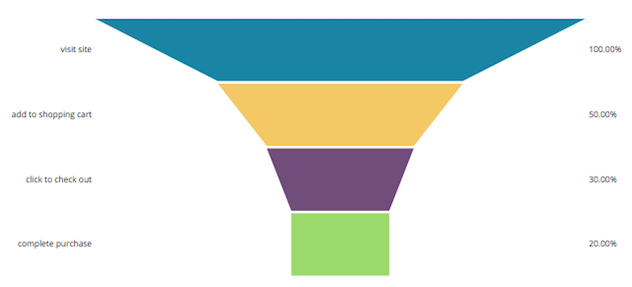
\includegraphics[width=\textwidth-10pt]{book-text/funnel.png}

There are actually three important funnel analyses to be done above:

\begin{itemize}
\item page view to add-to-bag user flow
\item page view to add-to-bag per recommendation
\item add-to-bag to complete purchase
\end{itemize}

The first funnel is merely understanding at a high level, what percentage of users take each step in the above flow. This is a high level measure of your website optimization, the general interestingness of your product offering, and the quality of your user leads.

The second funnel is more fine-grained to take into consideration the recommendations themselves. As mentioned above in the propensity scoring, users can only proceed through the funnel for a particular item if they're shown the item. This intersects with these ideas of funnels because you want to understand at a high level how certain recommendations correlate with funnel drop-off, but also when using a recommender system, the confidence in your recommendations should correlate well with the funnel metrics. We will return to this more in detail later when we discuss loss functions, but for now you should remember to think of different categories of recommendation-user pairs and how their funnels may look compared to average.

Finally, add-to-bag to completion. This actually isn't part of the RecSys problem, but should be on your mind as a Data Scientist or Machine Learning engineer trying to improve the product. **No matter how good your recommendations are, this funnel may destroy any of your hard work.** Before working on a recommender problem, you should almost always investigate the funnel performance in getting a user from add-to-bag to check-out-completed. If there's something cumbersome, or difficult about this flow, it will almost certainly provide a bigger bang-for-your-buck to fix this, than to improve recommendations. Investigate the drop-offs, do user-studies to understand what might be confusing, work with product and engineering to ensure everyone is aligned on this flow before you start building a recommender for e-commerce.

\section{Business insight and what people like}

In the above example from Bookshop.org, we notice that *Top Sellers of the Week* is the primary carousel on the page. Recall our earlier work on \lstinline{get_most_popular_recs}, this is simply that recommender but applied to a specific Collector–one that only looks in the last week. 

This carousel is an example of a recommender providing business-insight, in addition to driving recommendations. A common mission of a growth team is to understand weekly trends and KPIs, often things like weekly-active-users, and new signups. For many digital-first companies, growth teams are additionally interested in understanding the primary drivers.

Let's take an example: as of the writing of this, the Netflix show ***Squid Game*** became Netflix' most popular series of all time, breaking a huge number of records in the process. Squid Game achieved 111 Million viewers in the first month. Most obviously, *Squid Game* needs to be featured in *Top Shows of the Week* or *Hottest Titles* carousels, but what else does a breakout hit like this matter?

The first important insight companies almost always ask for is **attribution**–if the numbers go up in a week, what led to that? Is there something important or special about launches that drove additional growth? How can we learn from that to do better in the future? In the case of *Squid Game*–a foreign-language show that saw massive interest with an English-speaking crowd–executives might take away the inclination to invest more in shows from South Korea, or subtitled shows with high-drama. The flip side of this coin is also important, when growth metrics lag, executives nearly always ask why–being able to point to what was the most popular, and how it may have deviated from expectation, helps a lot.

The other important insight can feed back into recommendations; during exciting debuts like *Squid Game*, it's easy to get caught up in the excitement as you see all your metrics go up and to the right, but might this negatively effect things also? If you have a debut show the same week or two as *Squid Game's* you'll be less enthusiastic about all this success. Overall, successes like this usually drive *incremental* growth which is great for business, and in total, metrics will all probably look up. Other items however may have less successful launches due to a zero-sum game amongst the core user base. This can have a negative effect on longer term metrics, and even can make later recommendations less effective. 

Later, we will learn about diversity of recommendations. There are a large number of reasons to care about diversifying your recommendations, but here we observe one which is to increase the overall matching valence of your users with items. As you keep a broad base of users highly engaged, you increase your future opportunity for growth.

\vspace{10pt}
\colorbox{almond}{\parbox{\textwidth-20pt}{ \emph{Incremental gains} is a term modified from economics and put to use in growth marketing and growth analytics. Incremental gains refer to a margin of increase in addition to the gains expected from an expended effort. A simple example would be a business that usually adds a user for ever \$100 in marketing spend, gets some positive press, and the next week they get a user for every \$80 in marketing spend. If they keep their marketing budget fixed that week at \$1600, they would get 20 new users instead of 16; an incremental gain of 4 users. This is especially common when testing new treatments or programs.
}}

\vspace{10pt}
Finally, beyond surfacing the trending hits, another benefit of knowing what's really hot on your platform or service, is advertising. When a phenomenon starts, there can be a huge advantage in priming the pump, i.e. making noise and publicity of the success. This sometimes leads to a network effect, and in the days with viral content and easy distribution, this can have multiplier effects on your platform's growth.

\chapter{Mathematical Considerations}
\label{ch:math}

\section{Zipf's laws in RecSys and the Matthew Effect}

In a great many applications of machine learning, a caveat is given early, that the distribution of observations of unique items from a large corpus is modeled by Zipf's law. In recommendation systems, the \emph{Matthew Effect} appears in the popular item's click rates, or the popular user's feedback rates. 

Simply, the Matthew Effect–or popularity bias–states that the most popular items continue to attract the most attention and widen the gap with other items. Take for example the MovieLens dataset, an extremely popular dataset for benchmarking recommendation systems[link to MovieLens info], in [[Jenny Sheng 2020]\url{https://jennysheng.com/jenny-sheng-iw-fall-2020.pdf}] they observe the following behavior for number of movie ratings:

\vspace{10pt}
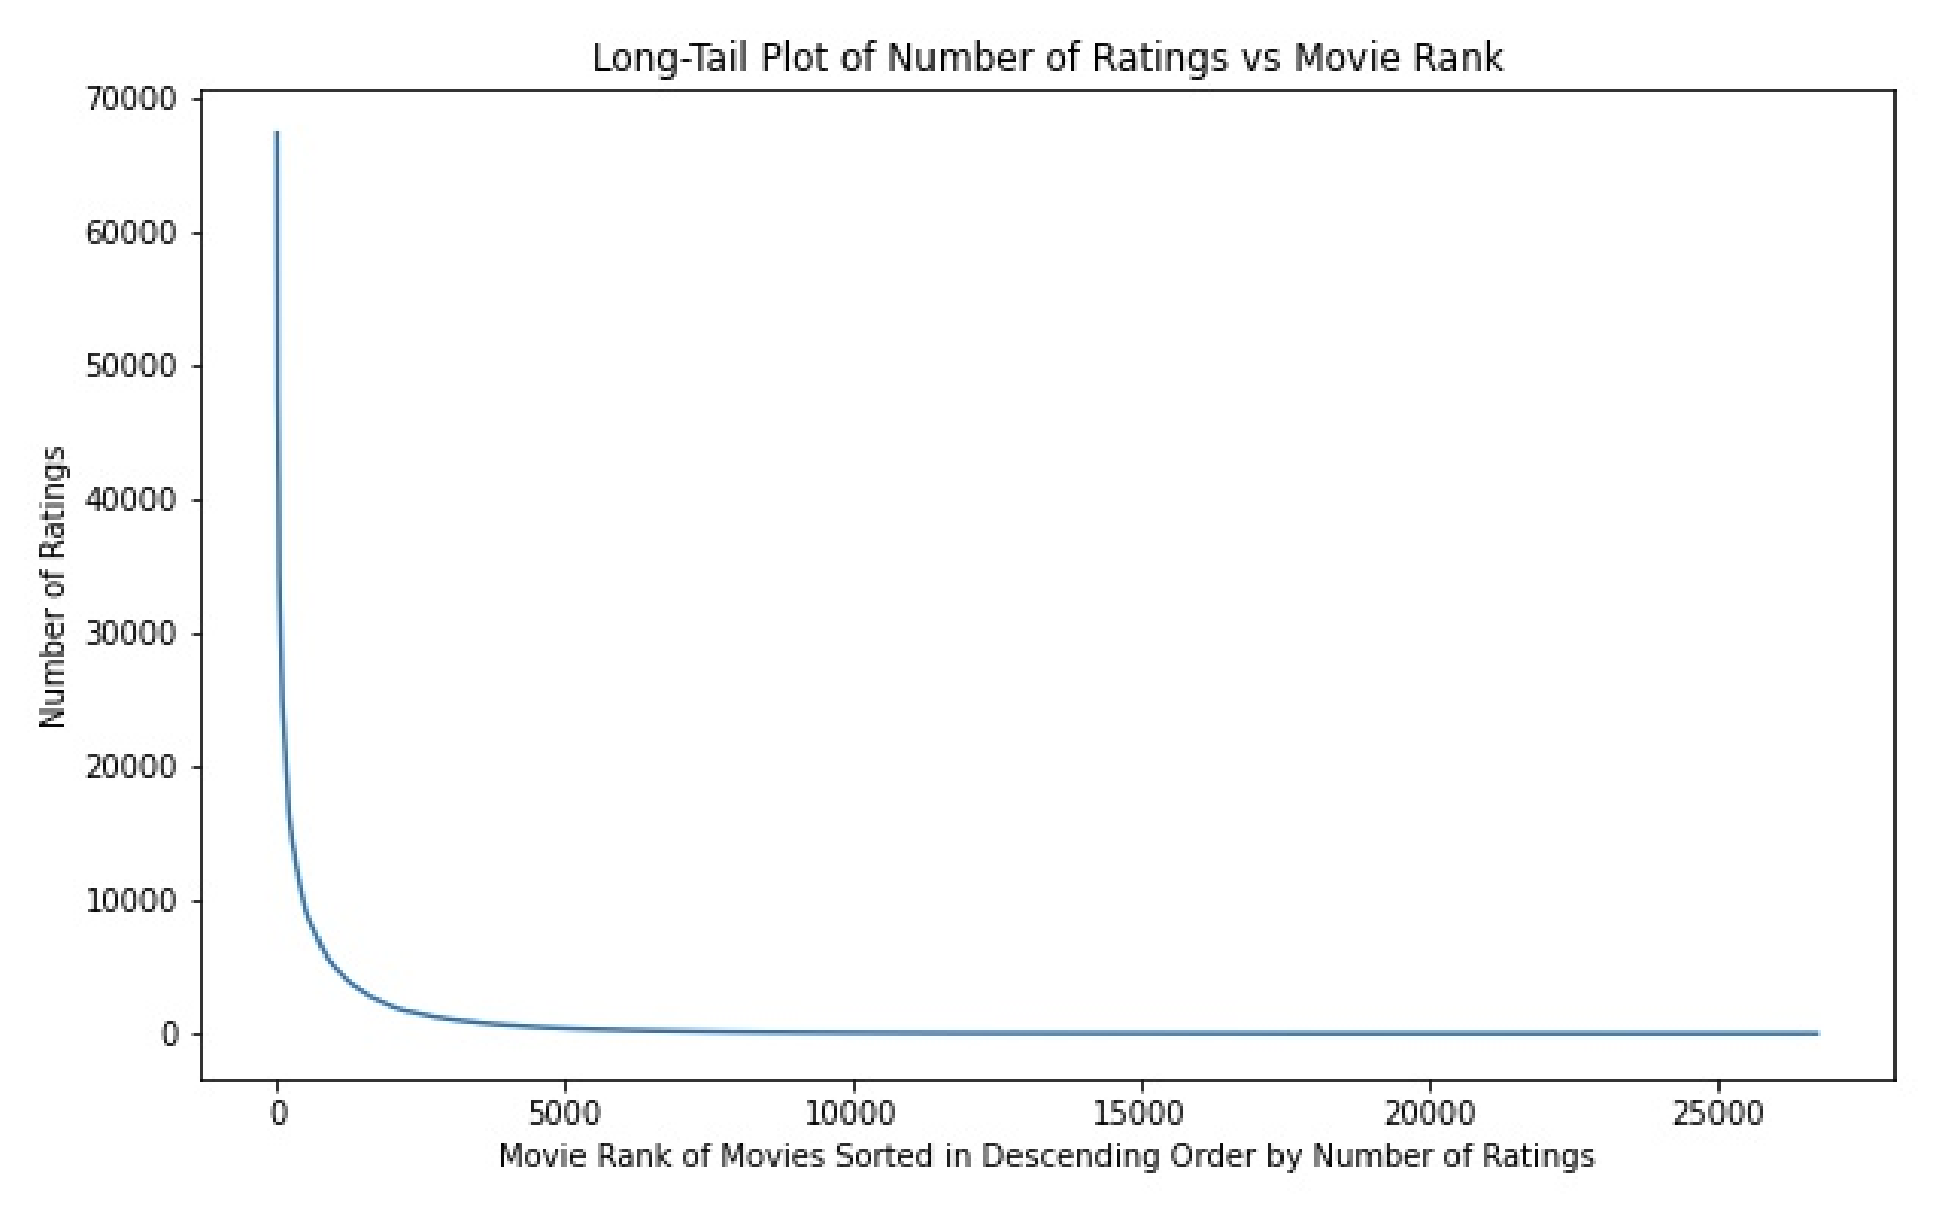
\includegraphics[width=\textwidth-10pt]{book-text/zipfian-moverank.png}

At first glance this behavior is obvious and stark, but is it a problem? Let's assume our recommender will be built as a user-based CF model–as alluded to in \ref{ch:user-item}–then how might these distributions effect the recommender?

Let the probability mass function be described by the simple Zipf's law:

\begin{equation}
    f(k, M) = \frac{1/k}{\sum^M_{n=1}(1/n)}    
\end{equation}


for $M$ number of tokens in the corpus (in the above examples number of movies), $k$ is the rank of a token when sorted by number of occurrences. 

Let's consider users $A$ and $B$, with $N_A = \mathcal{I}_A$  and $N_B = \mathcal{I}_B$ ratings respectively, Observe that the probability of $V_i$, the $i$'th most popular video, appearing in $\mathcal{I}_X$ for some user $X$ is given by:
\begin{equation}
    P(i)=\frac{f(i,M)}{\sum^M_{j=1}f(j,M)}=\frac{1/i}{\sum^M_{j=1}1/j}
\end{equation}

and thus the joint probability of an item appearing in two user's ratings is:

\begin{equation}
  P(i^2)=\left(\frac{1/i}{\sum^M_{j=1}1/j}\right)^2.  
\end{equation}

This becomes important when one also considers that our, yet unstated, definition of user-based collaborative filtering, is based on similarity in user's ratings sets–\emph{number of jointly rated items by two users, divided by the total number of items rated by either.}

Taking this definition, we can for example, compute the similarity score for one shared item amongst $A$ and $B$:

\begin{equation}
    \sum^M_{i=1} \frac{P(i^2)}{\| \mathcal{I}_A \cup \mathcal{I}_B \|},
\end{equation}

and the average similarity score of two users is generalized to:

\begin{equation}
    \sum^{\min(N_A,N_B)}_{t=1}\left(\prod_{i_k=i_{k-1}+1}^{t-1}\sum^M_{i=1} \frac{P({i_k}^2)}{\frac{\| \mathcal{I}_A \cup \mathcal{I}_B \|}{t}}\right).
\end{equation}

These combinatorial formulas indicate not only the relevance of the Zipfian in our algorithms, but we see an almost direct effect on the output of scores. Consider the experiment from [(Wang, Wang, and Zhang 2019)]\url{https://arxiv.org/abs/1909.12798}; for LastFM users, the authors demonstrate average similarity scores for pairs of users, and they find this Matthew Effect persists into the similarity matrix:

\vspace{10pt}
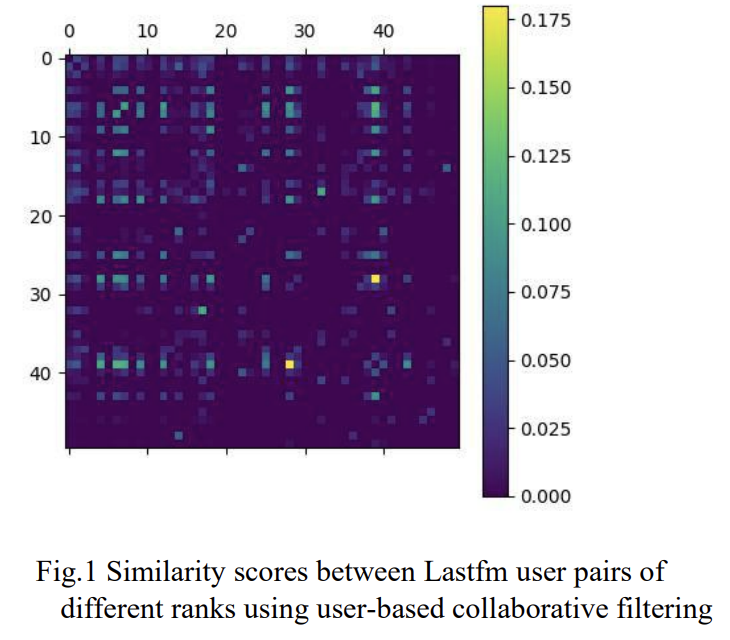
\includegraphics[width=\textwidth-10pt]{book-text/lastfm-matthew-effect.png}

While these results might seem scary, we'll observe later via diversity-aware loss functions that we can mitigate some of this. An even simpler way, is to use downstream sampling methods, which we will discuss as part of our explore-exploit algorithms. Finally, the Matthew Effect is only the first of two major impacts of this Zipfian–let's turn our attention to the second.


\section{Sparsity}

We now must reckon with sparsity. As the ratings skew more and more towards the most popular items, the least popular items a starved for data and recommendations, which is called \emph{Data Sparsity.} This connects to the linear algebraic definition of sparsity, mostly zeros or not populated elements in a vector, when you consider again our user-item matrix less popular items constitute columns with very few entries–these are sparse vectors. Similarly, at scale we see that the Matthew effect pushes more and more of the total ratings into certain columns, and the matrix becomes sparse in the traditional mathematical sense. For this reason, sparsity is an extremely well known challenge for recommendation systems. 

Like above, let's consider the implication on our collaborative filtering algorithms from these sparse ratings. Again observe that the probability of $V_i$, the $i$'th most popular item, appearing in $\mathcal{I}_X$ for some user $X$ is given by:

\begin{equation}
    P(i)=\frac{f(i,M)}{\sum^M_{j=1}f(j,M)}=\frac{1/i}{\sum^M_{j=1}1/j}
\end{equation}

then 

$$(M-1)*P(i)$$

is the expected number of other users which click the $i$'th most popular item, so summing over all $i$ yields the total number of other users that will share a rating with $X$:

\begin{equation}
    \sum_{i=1}^M (M-1)*P(i)
\end{equation}

Again, as we pull back to the overall trends, we observe this sparsity sneaking into the actual computations for our collaborative filtering algorithms, consider the trend of users of different ranks, and how much their rankings are used to 'collaborate' in other user's rankings:

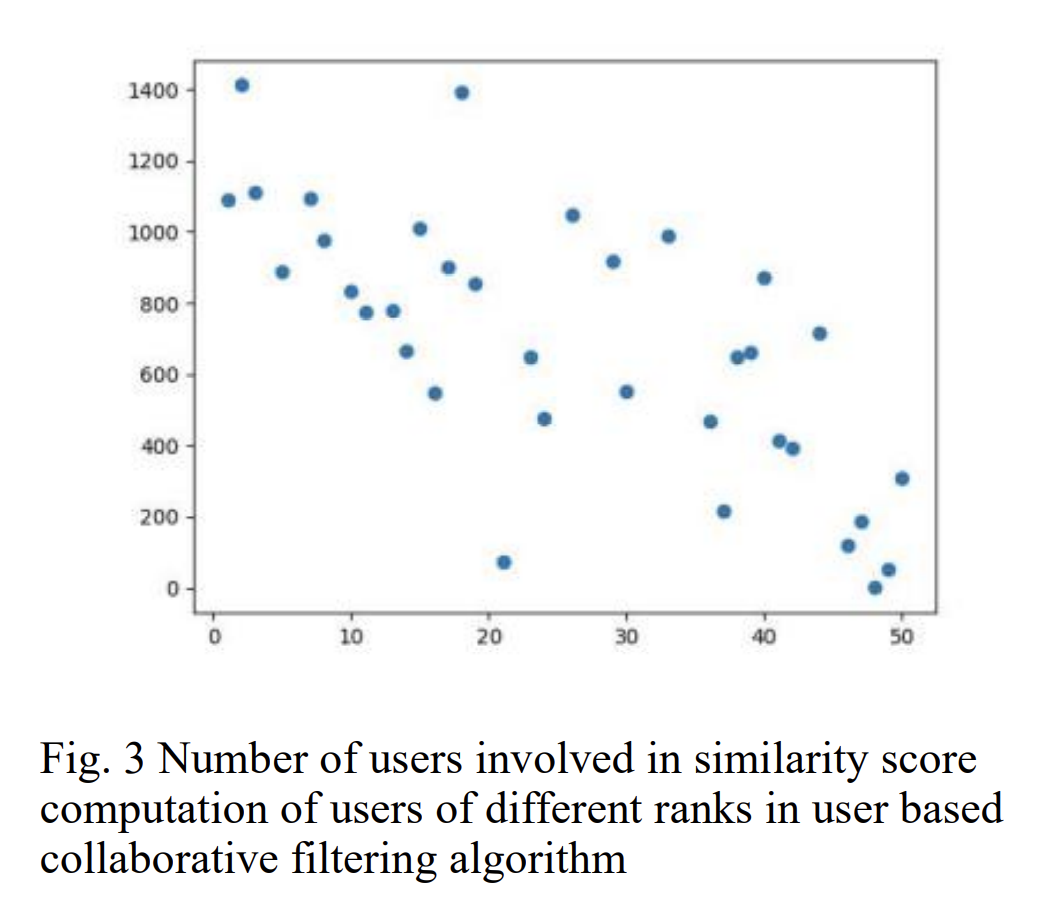
\includegraphics[width=\textwidth-10pt]{book-text/user-sim-counts.png}

We see that this is an important result to always beware–sparsity pushes emphasis onto the most popular users, and has the risk of making your recommender myopic. 

\subsection{Item-based collaborative filtering}

While the equations are different, everything above applies similarly to item-based collaborative filtering. We see similarity in items exhibit the same inheritance of the Zipfian in their scores, and we see items consulted in the collaborative filtering process drops off by rank. 

\section{User Similarity for Collaborative filtering}

In mathematics, it's most common to hear discussion of \emph{distances}–even back to the Pythagorean theorem, we are taught to think of relationships between points as distances, or dissimilarity. Indeed, this fundamental idea is canonized in mathematics as part of the definition of a metric:
\begin{itemize}
    \item $d(a,c)\leq d(a,b)+d(b,c)$
\end{itemize}


In machine learning; we often instead concern ourselves with the notion of similarity–an extremely related topic. In many cases, one can directly pass back and forth between similarity and dissimilarity; when $d:X\times X\rightarrow [0,1]\subset\mathbb{R}$ then we often define:

\begin{equation}
    Sim(a,b):=1-d(a,b)
\end{equation}

This may seem like a needlessly precise statement, but in fact we'll see that there are a [variety of options for how to frame similarity]\url{https://en.m.wikipedia.org/wiki/Similarity_measure}. Furthermore, sometimes we even formulate similarity measures where the associated distance measure does not establish a metric on the set of objects. These so-called pseudo-spaces can still be incredibly important, and we'll see where they come up in the later section on latent spaces. 

In the literature, you'll find a very common practice of papers starting by introducing a new similarity measure, and then training a model you've seen before on the new similarity measure. As we'll see, choices in how you choose to relate objects(users, items, features, etc.) can have a large effect on what your algorithms learn. 

For now, let's laser in on some specific similarity measures. Consider a classic ML problem of clustering; we have a space (usually $\mathbb{R}^n$) in which our data is represented and we are asked to partition our data into sub-collections of the population and assign these collections names. Frequently, these collections are intended to capture some meaning, or at the very least be useful for summarizing the collection elements' features. When you do that clustering, you frequently are considering points near to one another in that space. Further, if you're given a new observation, and asked to assign it to a collection as an inference task you normally compute the new observation's \emph{nearest neighbors}. This could be the k-nearest neighbors, or simply the nearest neighbor amongst cluster centers; either way, your task is to use the notion of similarity to associate. In collaborative filtering, this same notion is used to relate a user for whom you wish to make recommendations, to those you already have data from. 

So how may we define similarity for our users in collaborative filtering? They're not obviously in the same space, so our usual tools seem to be lacking. 

\subsection{Pearson correlation}

Our original formulation of Collaborative Filtering was to say that users with similar taste collaborate to recommend items for each other. Let two users $A$ and $B$, have a set of co-rated items–simply the set of items with ratings from each–written $\mathcal{R}_{A,B}$, and a rating of item $x$ by user $A$ written as $r_{A,x}$, then 

\begin{equation}
    \sum_{x\in \mathcal{R}_{A,B}}(r_{A,x}-\bar{r}_A)
\end{equation}

is the average deviation from $A$'s average rating over all of its co-rated items with $B$. If we think of these ratings as a random variable, and consider the analog for $B$, then the correlation between the jointly distributed variables, i.e. the population covariance, is our \emph{Pearson correlation:}

\begin{equation}
USim_{A,B}=\frac{\sum_{x\in \mathcal{R}_{A,B}}(r_{A,x}-\bar{r}_A)(r_{B,x}-\bar{r}_B)}{\sqrt{\sum_{x\in \mathcal{R}_{A,B}}(r_{A,x}-\bar{r}_A)^2} \sqrt{\sum_{x\in \mathcal{R}_{A,B}}(r_{B,x}-\bar{r}_B)^2}}    
\end{equation}

It's extremely important to keep in mind a few details here:

- This is the similarity of the jointly distributed variables describing the users' ratings
- We compute this via all co-rated items, so user similarity, is defined via item-ratings
- This is a pairwise similarity measure taking values in $[-1,1]\in \mathbb{R}$

\subsection{Ratings via similarity}

Now that we've introduced user-similarity, let's use it!

For a user $A$, and item $x$, we can estimate the rating via similar users' ratings:

\begin{equation}
    Aff_{A,i}=\bar{r}_A+\frac{\sum_{U\in \mathcal{N}(A)}USim_{A,U}*(r_{U,i}-\bar{r}_A)}{\sum_{U\in \mathcal{N}(A)}USim_{A,U}}
\end{equation}

This is the prediction for user $A$'s rating of item $x$, which takes $A$'s average adjusted rating of the similarity-weighted average ratings of all of $A$'s neighbors. In other words: $A$'s rating will probably be the average of people like $A$'s rating, adjusted to how generous $A$ is with ratings in general.

But wait! What's $\mathcal{N}(A)$? It's the neighborhood of $A$, via our $USim$ definition above. How many neighbors? How do you pick those neighbors? These will be the subject of later chapters; for now, assume they're $k$-nearest neighbors and assume some hyperparameter tuning is used to determine a good value for $k$.

\subsection{Fun aside:}

You might wonder, "does this Pearson correlation yield a metric space under some transformation?". The answer is yes, but it's a bit more complicated than our simple definition above. While the above can get us a distance, it's not good enough to get us a metric space, without a more novel transformation.

In particular, for $P(A,B)$ the above defined correlation, then $1-P(A,B)$ yields a distance that satisfies all metric properties *except* the triangle inequality. There are several known ways to adjust this though: $\sqrt{1-P(A,B)^2}$ being the most common. For a survey, see ([Dongen and Enright, 2012]\url{https://arxiv.org/pdf/1208.3145.pdf})

\section{Explore–exploit as a RecSys}

In the previous we saw two ideas, slightly in contrast to one another:

\begin{itemize}
\item The MPIR, a simple easy to understand recommender
\item The Matthew effect in recommendation systems, and it's runaway behavior in distributions of ratings
\end{itemize}

By now, it's likely that you realize that the MPIR will amplify the Matthew effect, and that the Matthew effect will drive the MPIR to the Trivial recommender in the limit. This is the classic difficulty of maximizing a loss function with no randomization–it very quickly settles into a mode.

This problem–and many others like it–encourage some modification to the algorithm to prevent this failure mode, and continue to expose the algorithm and users to other options. The basic strategy for \emph{explore-exploit schemes,} or \emph{multi-armed bandits} as they're called, is to take not only the outcome-maximizing recommendation, but also a collection of alternative \emph{variants,} and randomly determine which to use as response. 

Taking a step back: given a collection of variant recommendations, or \emph{arms}, $A$, for which the outcome of each recommendation is $y_t$, and we have a prior reward function $R(y_t)$. The bandit–called an \emph{agent} in this literature–would like to maximize $R(y_t)$, but the agent doesn't know the distribution of the outcomes $Y_{a\in A}$. The agent thus assumes some prior distributions for $Y_{a\in A}$, and then collects data to update those distributions; after sufficient observations, the agent can estimate the expected values of each distribution, $\mu_{a\in A}=\mathbb{E}(\mathcal{R}(Y_a))$. If the agent was able to confidently estimate these reward values, the recommendation problem would be solved: at inference, the agent would simply estimate the reward values for all variants for the user, and select the reward-optimizing \emph{arm.} This is of course ridiculous in totality, but the basic idea is useful nonetheless: hold prior assumptions about what will be greatest expected reward, and explore alternatives with some frequency to continue to update the distributions and refine your estimators.

\subsection{$\epsilon$-greedy}

So how often should you explore vs. use your reward-optimizing arm? The first best algorithm is $\epsilon$-greedy; for $\epsilon \in (0,1)$, at each request the Agent has probability $\epsilon$ of choosing a random arm and probability $1-\epsilon$ of selecting the currently highest estimated reward arm.

Let's take the MPIR and slightly modify it to include some exploration. 

\begin{lstlisting}[language=Python]
import random

def get_item_popularities() -> Optional[Dict[str, int]]:
	...
		return item_choice_counts # Dict of pairs: (item-identifier, count item chosen)
  return None

def get_most_popular_recs_ep_greedy(
	max_num_recs: int, 
	epsilon: float
) -> Optional[List[str]]:
	assert epsilon<1.0
	assert epsilon>0

	items_popularity_dict = get_item_popularities() # type: Optional[Dict[str, int]]
	if items_popularity_dict:
		sorted_items = sorted(
			items_popularity_dict.items(), 
			key=lambda item: item[1]),
			reverse=True,
		)
		top_items = [i[0] for i in sorted_items]
		recommendations = []
		for i in range(max_num_recs): # we wish to return max_num_recs
			if random.random()>epsilon: # if greater than epsilon, exploit
				recommendations.append(top_items.pop(0))
			else: # otherwise, explore
				explore_choice = random.randint(1,len(top_items))
				recommendations.append(top_items.pop(explore_choice))
		return recommendations
  return None
\end{lstlisting}

The only modification to our MPIR is that now we have two cases for each potential recommendation from our \lstinline{max_num_recs}; if a random probability is less than our $\epsilon$ then we proceed as before and select the most-popular, otherwise we select a random recommendation. 

Note that we're interpreting maximization of reward as selecting most-popular items. This is an important assumption, and as we move into more complicated recommenders, this will be the crucial assumption that we modify to get different algorithms and schemes.

\paragraph{Collector}

The collector here need not change, we still want to get the item popularities first.

\paragraph{Ranker}

The ranker also does not change! We begin by ranking the possible recommendations by popularity.

\paragraph{Server}

If collector and ranker remain the same, then clearly the server is what must be adapted for this new recommender. This is the case, instead of taking the top items to fill \lstinline{max_num_recs} we now utilize our $\epsilon$ to determine at each step if the next recommendation added to our list should be next in line from the ranker, or a random selection. Otherwise, we adhere to the same API schema, and return the same shape of data.

\subsection{What should $\epsilon$ be?}

In the above, $\epsilon$ is a fixed number for the entire call, but what should the value be? This is actually an area of great study and the general wisdom is to start with large $\epsilon$ (to encourage more exploration) and then reduce over time. The rate at which you decrease it, the starting value, and so on, require serious thought and research. Additionally, it can be tied into your prediction loop and be part of the training process.

\section{The NLP-RecSys relationship}

Let's utilize some intuition from a different area of Machine Learning, Natural Language Processing. One of the fundamental models in NLP is word2vec; a sequence–based model for language understanding that utilizes the words which co-occur in sentences together. 

For skipgram-word2vec, the model takes sentences of words, and attempts to learn the implicit meaning of words via their co-occurrence relationships with other words in those sentences. Each pair of co-occurring words, constitutes a sample that is 1-hot encoded and sent into a vocabulary-sized layer of neurons, with a bottleneck layer, and a vocabulary-sized output layer for probabilities that words will occur.

Via this network, we reduce the size of our representation to the bottleneck dimension, and thus find a smaller dimensional representation of all our words than the original corpus-sized 1-hot embedding. The thinking is that similarity of words can now be computed via vector similarity in this new representation space. 

Why is this related to recommendation systems? Well, because if we take the ordered sequence of user-item interactions, e.g. the sequence of movies a user has rated, you can utilize the same idea from word2vec to find item similarity instead of word similarity. In this analogy, the user history is the 'sentence'.

Previously, using our collaborative filtering similarity, we decided that similar users, can help inform what a good recommendation for a user should be. In this model we instead are finding item-item similarity, so instead we assume that items similar to those a user previously liked, they will also like. 

\subsection{Vector search}

We have build a collection of vector representations of our items, and we claim that similarity in this space (often called a latent-space, representation space, or ambient-space) means similarity in 'likeability' to users.

To convert this to a recommendation, consider a user $A$ with a collection of previously liked items $\mathcal{R}_A$, and consider $\mathcal{A}=\lbrace v_x | x\in \mathcal{R}_A\rbrace$ the set of vectors associated to those items in this latent-space. We are looking for a new item $y$ that we think is good for $A$.

One simple way is to take the closest item to the average of those that $A$ likes:

\begin{equation}
	\textrm{argmin}_y\left\lbrace d(v_y,avg(\mathcal{A}))\mid y\in \textrm{Items}\right\rbrace,
\end{equation}

where $d(-,-)$ is a distance function in the latent-space (usually cosine-distance).

This essentially treats all of $A$'s ratings equally and suggests something near those. In practice, this is often fraught. First, you could weight them by rating:

\begin{equation}
	\textrm{argmin}_y\left\lbrace d(v_y,\frac{\sum_{v_x\in\mathcal{A}}r_x}{|\mathcal{R_A}|})\mid y\in \textrm{Items}\right\rbrace,
\end{equation}

which potentially can improve the representativeness of the user feedback in the recommendations. Alternatively, you might find that a user rates movies across a variety of genre and themes. Averaging here will definitely lead to worse results, so maybe you which to simply find recommendations similar to 1 movie the user liked weighted by that rating:

\begin{equation}
	\textrm{argmin}_y\left\lbrace \frac{d(v_y,v_x)}{r_x}\mid y\in \textrm{Items}, v_x\in\mathcal{A}\right\rbrace.
\end{equation}

Finally, you may even want to do this process several times for different items a user liked to get $k$ recommendations:

\begin{equation}
	\textrm{min-}k \left\lbrace \textrm{argmin}_y\left\lbrace \frac{d(v_y,v_x)}{r_x}\mid y\in \textrm{Items}\right\rbrace\mid v_x\in\mathcal{A}\right\rbrace.
\end{equation}

Now we have $k$ recommendations, each is very similar to something that the user has liked, and is weighted by how much they liked it. And this approach only utilized an implicit geometry of the items formed by their co-occurrences. 

Latent-spaces and the geometric power that comes with them for recommendations will be a through-line for the rest of the book. We will often formulate our loss functions via these geometries, and exploit the geometric intuition to brainstorm where to expand our technique next. 

\subsection{Aside: Nearest-neighbors search}

A reasonable question to ask is "how do I get these vectors that minimize this distance"? In all of the above schemes, we are computing many distances and then finding minimums. In general, the problem of nearest-neighbors is an extremely important and well studied question. While finding the exact nearest-neighbors can sometimes be very slow; a lot of great progress has been made on Approximate Nearest Neighbors search. These algorithms not only return very close to the actual nearest-neighbors, but they perform orders of complexity faster. In general, when you see us (or in many papers) computing an $\textrm{argmin}$ over some distances, there's a good chance approximate nearest neighbors is what's used in practice.



In this section, let's begin our discussion of the core elements of a system that is needed to serve recommendations at industrial scale. In theory, a recommendation system is a collection of math formulae which can take historical data about user-item interactions, and return probability estimates for user-item pair's affinity. In practice, a recommendation system is 5, 10, maybe 20 software systems, communicating in real-time, working with limited information, restricted item-availability, and perpetually-out-of-sample behavior, to ensure the user sees \textit{something.}

This section is heavily influenced by the writing of Karl Higley and Eugene Yan.

\section{Online vs Offline}

In Machine Learning systems, the most frequent terminologies you'll encounter for the two sides of this paradigm are \emph{batch} and \emph{real-time}.
A \emph{batch process} is something that does not require user input, often has longer expected time periods for completion, and is able to have all the necessary data available simultaneously. Batch processes often include things like training a model on historical data, augmenting one data set with an additional collection of features, or computationally expensive data transformation. Another characteristic you see more in batch processes are that it works with the full dataset involved, not only a subset of the data sliced by time or otherwise.

A \emph{real-time} \emph{process} is characterized by something that is carried out at time of request, or said differently, something that is evaluated during the inference process. Examples include: providing a recommendation upon page load, updating 'next episode' after the user finishes the last, re-ranking recommendations after one has been marked 'not interesting'. Real-time processes are often resource-constrained because of the need for rapidity, but like many things in this domain, as the world's computational resources expand, we change the definition of resource-constrained.

Let's return to the previously introduced components–collector, ranker, server–and let's consider their roles in offline and online components. Recall:

\section{Collector}

The collector's role is to know what is in the collection of things that may be recommended, and the necessary features or attributes of those things.

\subsection{Offline Collector}

The offline collector has access to, and is responsible for the largest data sets. Understanding all user-item interactions, user-similarities, item-similarities, feature stores for users and items, and building indices for nearest neighbor lookup are all under the purview of the offline collector.

It's important to remember that the offline collector needs not only access and knowledge of these datasets, but also will be responsible for writing the necessary downstream datasets to be used in real time.

\subsection{Online Collector}

The online collector uses the information indexed and prepared by the offline collector, to provide real-time access to the parts of this data necessary for inference. This includes things like searching for nearest neighbors, augmenting an observation with features from a feature store, or full inventory catalog knowledge. 

One additional role the online collector may take on is encoding a request. In the context of a search recommender, we wish to take the query, and encode it into the 'search space' via an embedding model. For contextual recommenders, we need to encode the context into the 'latent space' via an embedding model also. 

\section{Ranker}

The ranker's role is to take the collection provided by the collector, and order some or all of them, according to a model for the context and user. The ranker actually gets two components itself, the \emph{filtering} and the \emph{scoring.}

Filtering can be thought of as the coarse inclusion and exclusion of items appropriate for recommendation. Usually characterized by rapidly cutting away a lot of potential recommendations that we definitely don't wish to show. A trivial example is not recommending items we know the user has already chosen in the past.

Scoring is the more traditional understanding of ranking: creating an ordering on potential recommendations with respect to the chosen objective function.

\subsection{Offline Ranker}

The offline ranker's goal is to facilitate filtering and scoring. An Important technology that will be discussed later is the \emph{Bloom Filter}. A bloom filter allows the offline ranker to do work in batch, so that filtering in real-time may happen much faster. An over simplification of this process would be to use a few features of the request to quickly select between subsets of all possible candidates; if this step can be made fast–in terms of computational complexity, and striving for something less than quadratic in the number of candidates–downstream complex algorithms can be made much more performant.

Second to the filtering step is the ranking step. In the offline component, ranking is training the model that learns how to rank items. As we will see later, learning to rank items to perform best with respect to the objective function, is at the heart of the recommendation models. Training these models, and preparing the aspects of their output, is part of the batch responsibility of the Ranker.

\subsection{Online Ranker}

The online ranker get's a lot of praise, but really utilizes the hard work of other components. The online ranker first does filtering, utilizing the filtering infrastructure built offline–for example an index lookup or a bloom filter application. After filtering, the number of candidate recommendations has been tamed, and thus we can actually come to the point: rank recommendations.

In the online ranking phase, usually a feature store is accessed to take the candidates and embellish them with the necessary details, and then a scoring and ranking model is applied. Scoring or ranking may happen in several independent dimensions, and then be collated into one final ranking. In the multi-objective paradigm, you may have several of these ranks associated to the list of candidates returned by a ranker.

\section{Server}

The server's role is to take the ordered subset provided by the ranker, ensure that the necessary data schema is satisfied–including essential business logic–and return the requested number of recommendations. 

\subsection{Offline Server}

The offline server is responsible for high level establishment of what are the hard requirements of recommendations returned from the system. In addition to establishing and enforcing schema, this can be more nuanced things like "never return this pair of pants when also recommending this top". Often waved off as "business logic"–the offline server is responsible for creating efficient ways to impose top level priorities on the returned recommendations. 

An additional responsibility for the offline server is handling things like experimentation. There's a good chance at some point you'll want to run online experiments to test out all the amazing recommendation systems you build with this book. The offline server is the place where you'll implement the logic necessary to take experimentation decisions, and provide the implications in a way the online server can use them in real time.

\subsection{Online Server}

The online server takes the rules, requirements, and configurations established, and makes their final application to the ranked recommendations. A simple example would be diversification rules; as we will see later, diversification of recommendations can have a significant impact on the quality of a user's experience. The online server can read the diversification requirements from the offline server, and apply them to the ranked list to return the expected number of diverse recommendations.

It's important to remember that the online server is the endpoint that other systems will be getting a response from. While it's usually where the message is coming from, much of the most complicated components in the system are upstream. Be careful to instrument this system in a way that when responses are slow, each system is observable enough that you can identify where those performance degradations are coming from.

\part{Retrieval}

\backmatter

% \bibliographystyle{plainnat}


\printindex

\end{document}
